
\section{Theorie}
\label{sec:Theorie}
\subsection{Dipole in Ionenkristallen}
Als Ionenkristall bezeichnet man einen Kristall, in dem positiv geladene Kationen und negativ geladene Anionen gemeinsam ein Kristallgitter bilden. Ein Beispiel für einen solchen Kristall ist Kaliumbromid, welcher aus Kalium-Kationen und Brom-Anionen aufgebaut ist. Diese ordnen sich abwechselnd nebeneinander in einem einfachen kubischen Kristallgitter an. 

Durch eine Dotierung des Ionenkristalls, beispielsweise durch Strontium, können im Kristall Dipole erzeugt werden. Im Falle von Kaliumbromid nehmen durch die Dotierung Strontium-Kationen die Gitterplätze der Kalium-Kationen ein.
Da die Strontium-Kationen im Gegensatz zum Kalium zweifach positiv geladen sind entstehen im Kristall lokale positive Ladungen, welche eine Ladungserschiebung angrenzender Kalium-Kationen zur Folge haben, um die Ladungsneutralität im Kristall zu erhalten. Die daraus resultierende Fehlstelle im Kristallgitter fungiert als lokale negative Ladung und kann somit mit dem doppelt positiv geladenen Strontium einen Dipol bilden. 
\subsection{Dipolrelaxation}
In ihrem Grundzustand und ohne äußere Anregung ist die räumliche Orientierung der Dipole zufällig, sodass durch die gleichmäßige Verteilung im gesamten Kristall das Gesamtdipolmoment verschwindet. Erst durch das Anlegen eines äußeren elektrischen Feldes über eine größere Zeit können sich die Dipole in Richtung des Feldes ausrichten. Wenn das äußere Feld nach Ausrichtung der Dipole ausgeschaltet wird, können die Dipole durch Verschiebung der Leerstellen die einheitliche Ausrichtung durch Feld wieder verlassen, was als Dipolrelaxation bezeichnet wird. Damit eine Leerstellenverschiebung im Kristall überhaupt möglich ist wird allerdings ein Mindestmaß an Energie im Kristall benötigt, welche als Aktivierungsenergie $W$ bezeichnet wird. Die Besetzung der Zustände im Kristall folgt der Boltzmann-Verteilung, sodass die Relaxationszeit $\tau$, also die mittlere Zeit bis ein Dipol seine Orientierung ändert, eine Temparaturabhängigkeit der Form:
\begin{equation}
\tau(T)=\tau_0\exp\left(\frac{W}{k_BT}\right)
\end{equation}
\begin{figure}
\centering
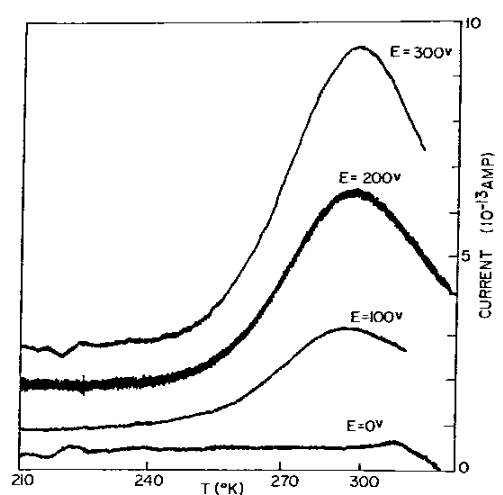
\includegraphics[width=0.5\textwidth,keepaspectratio]{Depolarisationsstrom}
\caption{Typische Verläufe des Depolarisationsstroms in Abbhängigkeit von der Temparatur für unterschiedliche elektrische Feldstärken \cite{fuller}.}
\label{fig:Depolarisationsstrom}
\end{figure}
mit der Boltzmann-Konstante $k_B$ und der charakteristischen Relaxationszeit $\tau_0=\tau(T=\infty)$ als materialspezifische Konstante. Durch die Relaxation der Dipole und die daraus folgende Ladungsverschiebung entsteht ein Strom, welcher an der Probe gemesssen werden kann. 
Dieser Strom ist temparaturabhängig und zeiigt typischerweise Verläufe wie in Abbildung \ref{fig:Depolarisationsstrom}.
\subsection{Berechnung der Aktivierungsenergie}
\subsubsection{Stromdichteansatz}
Um zunächst den Polarisationsstrom in Abhängigkeit von der Temparatur und daraus resultierend später die Aktivierungsenergie zu bestimmen gibt es verschiedene Ansätze. Die Debeye-Polarisation
\begin{equation*}
P=\frac{p^2E}{3k_BT}
\end{equation*}
mit dem Dipolmoment eines individuellen Dipols $p$ und dem elektrischen Feld $E$ gibt die durchnittliche Polarisation eines Dipols an. In Kombination mit der Zahl an teilnehmenden Dipolen sowie der Relaxationsrate $1/\tau(T)$ lässt sich nun die Stromdichte in Abhängigkeit von der Temparatur bestimmen:
\begin{equation}
I(T)=\frac{N_pp^2E}{3k_BT\tau_0}\exp \left( -\frac{1}{b\tau_0}\int^{T}_{T_0} \frac{dT'}{\tau(T')}\right)\exp\left(-\frac{W}{k_BT}\right)
\label{eq:IStromdichteansatz}
\end{equation}
Hierbei beschreibt $N_p$ die Ausgangszahl an ausgerichteten Dipolen und $b$ die Heizrate. 

Im Bereich der Kurve vor dem Maximum kann nun die Annahme getroffen werden, dass die Aktivierungsenergie sehr groß ist im Vergleich zur Energie $k_BT$ wodurch das Integral in der vorigen Gleichung verschwindet:
\begin{equation*}
 \int^{T}_{T_0} \frac{dT'}{\tau(T')}\approx 0
\end{equation*}
Nun ergibt sich durch logarithmieren der Gleichung der Zusammenhang:
\begin{equation}
\ln(I)=\frac{W}{k_BT}+\ln\left(\frac{N_pp^2E}{3k_BT\tau_0}\right)
\label{equ:1}
\end{equation}
Dadurch werden alle unbekannten Konstanten zusammangefasst und durch den linearen Zusammenhang zwischen dem Logarithmus des Stroms und dem Kehrwert der Temparatur lässt sich die Aktivierungsenergie durch eine einfache lineare Regression als Steigung $m$ der Gerade durch $W=mk_B$ berechnen. Das logarithmieren kompensiert außerdem die Tatsache, dass der Strom und nicht die Stromdichte gemessen wurde, da sich beide nach dem logarithmieren nur um eine Konstante unterscheiden.
\subsection{Polarisationsansatz}
Ein weiterer Ansatz lässt sich aus der Betrachtung der Gesamtpolarisation $P(t)$ herleiten. Durch das geschickte Umstellen der Gleichung
\begin{equation*}
\frac{dP}{dt}=\frac{P(t)}{\tau(T(t)}
\end{equation*}
und unter Ausnutzung der Tatsache, dass die Änderung der Gesamtpolarisation dem Depolarisationsstrom entspricht ($dP/dt=-I$), lässt sich die Gleichung
\begin{equation}
\tau(T)=\frac{\int^{\infty}_TI(T')dT'}{I(T)b}
\end{equation}
gewinnen. Aus dieser Gleichung lässt sich durch Einsetzen in die ursprüngliche Formel für die Relaxationszeit und umformen die Gleichung
\begin{equation}
\frac{W}{k_BT}=\ln\left(\frac{\int^{\infty}_TI(T')dT'}{I(T)b\tau_0}\right)
\label{equ:2}
\end{equation}
herleiten aus der wiederum per Ausgleichsrechnung die Aktivierungsenergie gewonnen werden kann. Im Gegensatz zu der ersten Formel lässt sich dies auf den gesamten Kurvenverlauf anwenden.
\section{Bestimmung der Relaxationsdauer}
Ein weiterer zu bestimmender Parameter ist die Relaxationsdauer $\tau_0$. Um diese zu bestimmen wird ausgenutzt, dass die Änderung des Stroms am Maximum bei der Temparatur $T_{max}$ verschwindet. Durch ableiten von Gleichung $\ref{eq:IStromdichteansatz}$ ergibt sich die Formel
\begin{equation}
\tau_0=\frac{k_BT_{max}^2}{Wb}\exp\left(-\frac{W}{k_BT_{max}}\right)
\label{equ:3}
\end{equation}